%%
%% ACM SIGPLAN Conference Template - Adaptive Gating with Variational Inference
%%
\documentclass[sigplan,screen]{acmart}
\setkeys{acmart.cls}{balance=false}

%% Bibliography settings
\AtBeginDocument{%
\providecommand\BibTeX{{%
Bib\TeX}}}

%% Packages for algorithms
\usepackage{algorithm}
\usepackage{algorithmic}
\usepackage{siunitx}

%% Allow page breaks inside equations
\allowdisplaybreaks

%% Rights management (replace with your data)
\setcopyright{acmlicensed}
\copyrightyear{2026}
\acmYear{2026}
\acmDOI{XXXXXXX.XXXXXXX}
\acmConference[Conference acronym 'XX]{Conference Title}{June 03--05, 2026}{City, Country}
\acmISBN{978-1-4503-XXXX-X/2026/06}

%% Submission ID (optional)
%%\acmSubmissionID{123-A56-BU3}

%% Citation style (uncomment for author-year)
%%\citestyle{acmauthoryear}

\begin{document}

%%
%% Title
%%
\title{Paper Title}

%%
%% Authors
%%
\author{Author 1}
\email{author1@email.com}
\orcid{0000-0000-0000-0000}
\affiliation{%
\institution{Institution}
\city{City}
\state{State}
\country{Country}
}

\author{Author 2}
\correspondingauthor
\email{author2@domain.com}
\affiliation{%
\institution{Institution}
\city{City}
\state{State}
\country{Country}
}

%% Short authors for page headers
\renewcommand{\shortauthors}{Author1 et al.}

%%
%% Abstract
%%
\begin{abstract}
We propose an accuracy-guided method for structural channel pruning in convolutional neural networks. The method learns a binary gate for each intermediate channel by combining a classification loss with a sparsity penalty and an optional entropy term. The sparsity penalty encourages fewer active channels, while the entropy term keeps gate probabilities from becoming deterministic too early. During training, we adjust the sparsity penalty using the validation accuracy gap relative to a dense reference model. The learned gate probabilities then guide permanent channel removal, and the resulting compact network is fine-tuned. Experiments with MobileNetV2 and ResNet-50 illustrate the trade-off between model size and classification accuracy.
\end{abstract}

%%
%% CCS Concepts
%%
\begin{CCSXML}
<ccs2012>
<concept>
<concept_id>10010147.10010257.10010293</concept_id>
<concept_desc>Computing methodologies~Neural networks</concept_desc>
<concept_significance>500</concept_significance>
</concept>
<concept>
<concept_id>10010147.10010178.10010179</concept_id>
<concept_desc>Computing methodologies~Supervised learning</concept_desc>
<concept_significance>300</concept_significance>
</concept>
</ccs2012>
\end{CCSXML}

\ccsdesc[500]{Computing methodologies~Neural networks}
\ccsdesc[300]{Computing methodologies~Supervised learning}

%%
%% Keywords
%%
\keywords{Adaptive Computation, Variational Inference, Gated Networks, Gumbel-Softmax, Layer Pruning, Dynamic Inference}

\received{Submission date}
\received[revised]{Revision date}
\received[accepted]{Acceptance date}

\maketitle

%%
%% Main text
%%

\section{Introduction}

Deploying convolutional neural networks under a limited parameter budget requires deciding which parts of the network can be removed while preserving predictive accuracy. Structural channel pruning addresses this problem by removing entire channels and the associated weights, yielding a narrower network. The central challenge is to determine how many channels can be removed and which ones to keep.

Prior work approaches channel selection and conditional execution from different perspectives. AutoPruner learns binary masks for filter removal, and DepGraph identifies groups of parameters that must be pruned together to preserve architectural consistency~\cite{luo2020autopruner,fang2023depgraph}. ConvNet-AIG uses binary gates to select which residual transformations to execute for each input~\cite{veit2018convnet}. We use binary gates during training to select intermediate channels for permanent removal. The resulting compact architecture is fixed across inputs.

Our method jointly learns the network weights and the opening probability of each channel gate. The training objective combines classification loss with a penalty on the expected number of active channels and an optional entropy term that encourages exploration during the search. When the entropy coefficient is positive, the two regularization terms admit an interpretation as a KL penalty toward a sparse Bernoulli prior. We adjust the sparsity coefficient using the validation accuracy gap to a dense reference model. Once the search is complete, the learned gate probabilities guide the construction of candidate subnetworks, and the selected subnetwork is fine-tuned after structural pruning.

Our contributions are threefold.

\begin{itemize}
    \item We formulate channel selection with learnable Bernoulli gates and relate the entropy and sparsity terms to a sparse Bernoulli prior.
    \item We use validation feedback to adjust the sparsity penalty during the search, increasing it when the accuracy gap is small and relaxing it when the gap becomes too large.
    \item We turn learned gate probabilities into compact, fixed architectures and examine the trade-off between parameter count and test accuracy using iterative pruning on MobileNetV2 and one-shot pruning on ResNet-50.
\end{itemize}

\section{Related Work}
\label{sec:related-work}

Feature selection and structured sparsification seek compact predictive
models by selecting input variables, hidden units, or channels during
training. Group sparse regularization penalizes groups of outgoing weights
to jointly learn network weights, select input features, and determine
hidden-layer widths~\cite{scardapane2017group}. Stochastic Gates (STG)
uses clipped Gaussian gates to learn a subset of input features while
penalizing the expected number of selected inputs~\cite{yamada2020feature}.
At the weight level, stochastic gates also allow the expected number of
nonzero parameters to be penalized through \(L_0\)
regularization~\cite{louizos2018learning}.

Structural channel pruning applies selection to intermediate feature maps
in convolutional networks. Network Slimming uses sparsity-regularized
batch normalization scaling factors~\cite{liu2017network}, while
AutoPruner learns binary filter masks jointly with network
weights~\cite{luo2020autopruner}. Discrimination-aware Channel Pruning
alternates greedy channel selection and parameter optimization using
auxiliary classification and feature-reconstruction
losses~\cite{zhuang2018discrimination}. CHIP evaluates channel independence
through the change in the nuclear norm of feature maps when a channel is
removed~\cite{sui2021chip}. DepGraph identifies groups of parameters that
must be pruned together to preserve architectural
consistency~\cite{fang2023depgraph}.

ConvNet-AIG uses input-dependent binary gates to select residual
transformations at inference time~\cite{veit2018convnet}. Herrmann et al.
learn channel gates using Gumbel-Softmax and a batch activation penalty
that targets a prescribed activation rate, supporting both fixed pruning
and input-dependent computation~\cite{herrmann2020channel}. Our method
also learns channel gates during training to obtain a fixed compact
network. Its objective penalizes expected channel activity and optionally
includes an entropy term that discourages gate probabilities from
becoming deterministic early in the search.

The amount of pruning can also be adapted during optimization.
DCP-Adapt determines the number of retained channels using a stopping
criterion based on the improvement in its selection
loss~\cite{zhuang2018discrimination}. AMC uses reinforcement learning to
search for layer-wise compression ratios~\cite{he2018amc}. Our method
adjusts the strength of the sparsity penalty during training using the
validation accuracy gap relative to a dense reference model. The learned
gate probabilities then guide permanent channel removal, followed by
fine-tuning of the compact network.

\section{Methodology}

\subsection{Channel-Wise Gating}

Consider a residual network with $L$ blocks. For clarity,
we describe a block with two transformations:
\begin{equation}
\mathbf{h}_l = a_{\theta,l}(\mathbf{x}_{l-1}),
\qquad
\mathbf{x}_l
=
s_l(\mathbf{x}_{l-1})
+
b_{\theta,l}(\mathbf{h}_l),
\end{equation}
where $a_{\theta,l}$ produces an intermediate feature map
with $C_l$ channels, $b_{\theta,l}$ maps these features to
the residual output, and $s_l$ is an identity shortcut or
a projection.

We introduce one binary gate for each intermediate channel:
\begin{equation}
g_{l,c}\in\{0,1\},
\qquad c=1,\ldots,C_l.
\end{equation}
The gated block becomes
\begin{equation}
\boxed{
\mathbf{x}_l
=
s_l(\mathbf{x}_{l-1})
+
b_{\theta,l}
\left(
\mathbf{g}_l\odot
a_{\theta,l}(\mathbf{x}_{l-1})
\right),
}
\end{equation}
where $\mathbf{g}_l=(g_{l,1},\ldots,g_{l,C_l})$ and
$\odot$ denotes channel-wise multiplication broadcast over
spatial dimensions.

When $g_{l,c}=0$, intermediate channel $c$ makes no
contribution to the subsequent transformation. Because
gating changes the intermediate representation rather than
the block output dimensions, the residual addition remains
dimensionally valid.

For a standard convolutional block, a permanently disabled
intermediate channel can be removed by deleting its output
filter from the preceding convolution, its associated
channel-wise normalization parameters, and the corresponding
input-channel slice of the following convolution.

Let
\begin{equation}
K=\sum_{l=1}^{L}C_l
\end{equation}
be the total number of gated channels, and let
$\mathbf{g}\in\{0,1\}^{K}$ collect all gate variables.

\subsection{Probabilistic Formulation}

For an input $\mathbf{x}$ and target $\mathbf{y}$, define
\begin{equation}
p_\theta(\mathbf{y},\mathbf{g}\mid\mathbf{x})
=
p_\theta(\mathbf{y}\mid\mathbf{x},\mathbf{g})
p(\mathbf{g}),
\end{equation}
where $p_\theta(\mathbf{y}\mid\mathbf{x},\mathbf{g})$ is the
predictive likelihood of the gated network and
$p(\mathbf{g})$ is a prior over channel masks.

The marginal likelihood is
\begin{equation}
p_\theta(\mathbf{y}\mid\mathbf{x})
=
\sum_{\mathbf{g}\in\{0,1\}^{K}}
p_\theta(\mathbf{y}\mid\mathbf{x},\mathbf{g})
p(\mathbf{g}).
\end{equation}

Exact evaluation requires summing over exponentially many
masks. We therefore introduce a variational distribution
\begin{equation}
q_\phi(\mathbf{g}\mid\mathbf{x})
=
\prod_{l=1}^{L}\prod_{c=1}^{C_l}
\operatorname{Bern}
\left(
g_{l,c}\mid r_{\phi,l,c}(\mathbf{x})
\right).
\end{equation}

Here, $r_{\phi,l,c}(\mathbf{x})$ is the probability of
activating channel $c$ in block $l$. A lightweight gating
network predicts the probabilities from features available
before the gated transformation:
\begin{equation}
\mathbf{r}_{\phi,l}(\mathbf{x})
=
\sigma\left(
h_{\phi,l}(\mathbf{z}_l(\mathbf{x}))
\right),
\end{equation}
where $h_{\phi,l}$ produces $C_l$ logits and $\sigma$ is the
element-wise sigmoid function.

The factorization assumes conditional independence of the
gate variables given the input. It does not imply that the
resulting feature channels are independent.

\subsection{Evidence Lower Bound}

Applying Jensen's inequality yields
\begin{equation}
\begin{split}
\log p_\theta(\mathbf{y}\mid\mathbf{x})
={}&
\log
\mathbb{E}_{q_\phi(\mathbf{g}\mid\mathbf{x})}
\left[
\frac{
p_\theta(\mathbf{y}\mid\mathbf{x},\mathbf{g})
p(\mathbf{g})
}{
q_\phi(\mathbf{g}\mid\mathbf{x})
}
\right]
\\
\geq{}&
\mathbb{E}_{q_\phi(\mathbf{g}\mid\mathbf{x})}
\left[
\log p_\theta(\mathbf{y}\mid\mathbf{x},\mathbf{g})
\right]
\\
&-
\operatorname{KL}
\left(
q_\phi(\mathbf{g}\mid\mathbf{x})
\,\Vert\,p(\mathbf{g})
\right).
\end{split}
\end{equation}

Thus, the evidence lower bound is
\begin{equation}
\begin{split}
\mathcal{L}_{\mathrm{ELBO}}
(\theta,\phi;\mathbf{x},\mathbf{y})
={}&
\mathbb{E}_{q_\phi(\mathbf{g}\mid\mathbf{x})}
\left[
\log p_\theta(\mathbf{y}\mid\mathbf{x},\mathbf{g})
\right]
\\
&-
\operatorname{KL}
\left(
q_\phi(\mathbf{g}\mid\mathbf{x})
\,\Vert\,p(\mathbf{g})
\right).
\end{split}
\end{equation}

For classification, the negative expected log-likelihood
is the expected cross-entropy loss.

\subsection{Binary Gate Sampling}

For brevity, write
$r_{l,c}=r_{\phi,l,c}(\mathbf{x})$ and define its logit
\begin{equation}
a_{l,c}
=
\log\frac{r_{l,c}}{1-r_{l,c}}.
\end{equation}

Sample independent noise variables
\begin{equation}
\epsilon^{(1)}_{l,c},
\epsilon^{(0)}_{l,c}
\sim\operatorname{Gumbel}(0,1).
\end{equation}
A Bernoulli gate can be sampled as
\begin{equation}
g^{\mathrm{hard}}_{l,c}
=
\mathbf{1}
\left[
a_{l,c}
+
\epsilon^{(1)}_{l,c}
-
\epsilon^{(0)}_{l,c}
>0
\right].
\end{equation}

We use the continuous relaxation
\begin{equation}
\widetilde{g}_{l,c}
=
\sigma\left(
\frac{
a_{l,c}
+
\epsilon^{(1)}_{l,c}
-
\epsilon^{(0)}_{l,c}
}{T}
\right),
\end{equation}
where $T>0$ is the temperature.

The straight-through gate is
\begin{equation}
g^{\mathrm{ST}}_{l,c}
=
\operatorname{stopgrad}
\left(
g^{\mathrm{hard}}_{l,c}
-
\widetilde{g}_{l,c}
\right)
+
\widetilde{g}_{l,c}.
\end{equation}

This construction uses binary masks in the forward pass
and gradients of the relaxation in the backward pass.
The resulting gradient estimator is biased.

\subsection{Channel Sparsity Regularization}

Choose a factorized Bernoulli prior:
\begin{equation}
p(\mathbf{g})
=
\prod_{l=1}^{L}\prod_{c=1}^{C_l}
\operatorname{Bern}(g_{l,c}\mid\pi_{l,c}).
\end{equation}

For a single gate, with posterior activation probability
$r$ and prior activation probability $\pi$,
\begin{equation}
\begin{split}
&\operatorname{KL}
\left(
\operatorname{Bern}(r)
\,\Vert\,
\operatorname{Bern}(\pi)
\right)
\\
&{}=r\log\frac{r}{\pi}
+
(1-r)\log\frac{1-r}{1-\pi}
\\
&{}=-H(r)
+
r\log\frac{1-\pi}{\pi}
-
\log(1-\pi),
\end{split}
\end{equation}
where
\begin{equation}
H(r)
=
-r\log r-(1-r)\log(1-r)
\end{equation}
is the Bernoulli entropy.

Motivated by this decomposition, define
\begin{equation}
\mathcal{R}_{\beta,\lambda}(\phi;\mathbf{x})
=
-\beta\sum_{l,c}H(r_{l,c})
+
\lambda\sum_{l,c}r_{l,c},
\end{equation}
where $\beta>0$ and $\lambda\geq0$.

The complete minimization objective is
\begin{equation}
\boxed{
\begin{aligned}
\mathcal{J}(\theta,\phi)
=
\mathbb{E}_{(\mathbf{x},\mathbf{y})\sim\mathcal{D}}
\Bigg[
&
\mathbb{E}_{q_\phi(\mathbf{g}\mid\mathbf{x})}
\left[
-\log p_\theta(\mathbf{y}\mid\mathbf{x},\mathbf{g})
\right]
\\
&-\beta\sum_{l,c}H(r_{l,c})
+\lambda\sum_{l,c}r_{l,c}
\Bigg].
\end{aligned}
}
\end{equation}

Minimizing $-\beta H(r)$ encourages uncertain gate
probabilities and discourages premature deterministic
decisions. The sparsity term penalizes the expected number
of active intermediate channels:
\begin{equation}
\mathbb{E}_{q_\phi(\mathbf{g}\mid\mathbf{x})}
\left[
\sum_{l,c}g_{l,c}
\right]
=
\sum_{l,c}r_{l,c}.
\end{equation}

This penalty measures expected channel count rather than
exact computational cost. Channels in different blocks
may have different costs because of their spatial
resolutions and convolutional dimensions.

\subsection{Interpretation as a Sparse Prior}

For fixed $\beta$ and $\lambda$, let all prior activation
probabilities equal
\begin{equation}
\boxed{
\pi=\sigma\left(-\frac{\lambda}{\beta}\right).
}
\end{equation}
Then
\begin{equation}
\beta\log\frac{1-\pi}{\pi}=\lambda.
\end{equation}
Consequently,
\begin{equation}
\begin{split}
-\beta H(r)+\lambda r
={}&
\beta\operatorname{KL}
\left(
\operatorname{Bern}(r)
\,\Vert\,
\operatorname{Bern}(\pi)
\right)
\\
&+\beta\log(1-\pi).
\end{split}
\end{equation}

Summing over all gates gives
\begin{equation}
\begin{split}
\mathcal{R}_{\beta,\lambda}(\phi;\mathbf{x})
={}&
\beta\operatorname{KL}
\left(
q_\phi(\mathbf{g}\mid\mathbf{x})
\,\Vert\,p_\pi(\mathbf{g})
\right)
\\
&+\beta K\log(1-\pi).
\end{split}
\end{equation}

The final term is constant with respect to $\theta$ and
$\phi$ when $\beta$ and $\lambda$ are fixed. Therefore,
the proposed objective is equivalent, up to an additive
constant, to the expected classification loss plus a
weighted KL divergence.

When $\beta=1$, this is the negative ELBO up to an additive
constant. For general $\beta>0$, it is a weighted
KL-regularized variational objective; it need not be the
negative of a standard ELBO.

Increasing $\lambda$ at fixed $\beta$ decreases $\pi$,
strengthening the prior preference for inactive channels.

\subsection{Interaction Between Entropy and Sparsity}

For a single gate, consider only its regularizer:
\begin{equation}
R(r)=-\beta H(r)+\lambda r.
\end{equation}
For $0<r<1$,
\begin{equation}
\frac{dR}{dr}
=
\beta\log\frac{r}{1-r}+\lambda.
\end{equation}
Setting this derivative to zero gives
\begin{equation}
r^*
=
\sigma\left(-\frac{\lambda}{\beta}\right).
\end{equation}
Moreover,
\begin{equation}
\frac{d^2R}{dr^2}
=
\frac{\beta}{r(1-r)}>0,
\end{equation}
so this is the unique minimizer of the regularizer.

Thus, the ratio $\lambda/\beta$ determines the preferred
activation probability in the absence of the prediction
loss. The learned gate probabilities also depend on how
each channel affects predictive performance.

A small entropy coefficient alone does not guarantee
deterministic gates, and a small sparsity coefficient alone
does not guarantee that all channels remain active.

\subsection{Adaptive Scheduling of the Sparsity Coefficient}
\label{sec:adaptive-sparsity}

For the one-shot procedure in Algorithm~\ref{alg:accuracy-guided-pruning},
let $A_t^{\rm ref}$ and $A_t$ denote the validation accuracies of the
dense reference and gated model at the same search epoch $t$.
The controller averages the last $w$ paired gaps:
\begin{equation}
\overline\Delta_t
=\frac{1}{w}\sum_{i=t-w+1}^{t}(A_i^{\rm ref}-A_i),
\qquad t\geq w.
\end{equation}

The coefficient $\lambda_t$ is used to train epoch $t$.
For the first $W$ warmup epochs, and until a full window is available,
$\lambda_{t+1}=\lambda_t$. Subsequently, after every epoch,
\begin{equation}
\lambda_{t+1}=
\begin{cases}
\min(\lambda_{\max},\lambda_t e^{\eta}),
& \overline\Delta_t\leq\delta_s,\\[2pt]
\max(\lambda_{\min},\lambda_t e^{-\eta}),
& \overline\Delta_t>\delta_h,\\[2pt]
\lambda_t, & \text{otherwise},
\end{cases}
\label{eq:one-shot-controller}
\end{equation}
where $0\leq\delta_s<\delta_h$ are accuracy tolerances and $\eta>0$
is the fixed log-step. Accuracies and tolerances are fractions.
This feedback rule preserves positivity and, before clipping to
$[\lambda_{\min},\lambda_{\max}]$, applies a fixed relative change.

The rule does not guarantee convergence or satisfaction
of the accuracy constraint at every epoch. In particular,
validation noise and delayed responses to regularization
can produce oscillations around the target accuracy drop.

For fixed $\beta$, updating $\lambda$ also updates the
corresponding prior:
\begin{equation}
\pi_t
=
\sigma\left(-\frac{\lambda_t}{\beta}\right).
\end{equation}
Increasing $\lambda_t$ makes the prior more sparse, while
decreasing it makes the prior less sparse. This is an
externally controlled prior schedule rather than
optimization of a single fixed-prior ELBO throughout
training.

\subsection{Structural Channel Pruning}

Input-dependent gates produce different masks for
different inputs. Permanent channel removal requires
selecting a fixed mask.

We estimate the average activation probability of each
channel on a representative calibration set
$\mathcal{D}_{\mathrm{cal}}$:
\begin{equation}
\overline{r}_{l,c}
=
\frac{1}{|\mathcal{D}_{\mathrm{cal}}|}
\sum_{\mathbf{x}\in\mathcal{D}_{\mathrm{cal}}}
r_{\phi,l,c}(\mathbf{x}).
\end{equation}

Channels satisfying
\begin{equation}
\overline{r}_{l,c}
<
\varepsilon_{\mathrm{prune}}
\end{equation}
are candidates for permanent removal, where
$\varepsilon_{\mathrm{prune}}\in(0,1)$ is a pruning
threshold.

For the intermediate-channel placement described above,
structural pruning removes the corresponding output
channels of $a_{\theta,l}$ and input channels of
$b_{\theta,l}$, together with associated channel-wise
parameters. The output dimensions of the residual branch
and shortcut remain unchanged.

This operation assumes compatible channel connectivity,
as in standard dense convolutions with channel-wise
normalization. Grouped convolutions and operations that
mix channels require additional structural constraints.

Pruning can be performed iteratively:
\begin{enumerate}
\item Train the gated network.
\item Estimate average channel activation probabilities.
\item Remove a selected set of low-probability channels.
\item Fine-tune and validate the reduced network.
\item Repeat while the desired accuracy--size trade-off
remains acceptable.
\end{enumerate}

Low average activation probability is a pruning heuristic,
not a guarantee that a channel is unnecessary for every
input. Predictive performance must therefore be evaluated
after structural removal.

Binary masking alone does not reduce the cost of
convolutions that have already been computed. Actual
computational savings require physical channel removal
or an execution backend that avoids inactive computations.
Any efficiency evaluation must also account for the cost
of the gating modules.

% BEGIN COMPACT PRUNING ALGORITHM
\paragraph{Algorithm overview.}
Algorithm~\ref{alg:accuracy-guided-pruning} specifies the one-shot
procedure with input-independent gates used for ResNet-50.
Here $T_s,T_r$ are the search and recovery budgets.
Section~\ref{sec:adaptive-sparsity} defines the controller, including
warmup, the paired averaging window, the fixed log-step and clipping.
The default automatic log-step is computed once and requires
$\lfloor T_s/3-W\rfloor\geq1$ and
$\lambda_{\min}\leq\lambda_0<\lambda_{\rm target}\leq\lambda_{\max}$.
Numerical training settings are given in
Section~\ref{sec:resnet-cifar-implementation}.

Let $(\theta_t,\phi_t)$ denote the saved search checkpoint, with
$\theta_t$ including the weights and corresponding BatchNorm statistics,
and $\phi_t$ the gate logits. The operator
$\operatorname{MakeMask}_{\geq1}(\phi_t)$ keeps all channels with $r>0.5$
in each group; if none qualify, it keeps one channel with maximal $r$.
This minimum can activate a channel closed in the original gated
validation. For each second-half checkpoint,
$\operatorname{Eval}_{\rm val}(\theta_t,m_t)$ measures validation accuracy
with the fixed mask, without updating weights or BatchNorm statistics;
no training or BatchNorm recalibration occurs during selection.
$\operatorname{Params}(m_t)$ counts the parameters of the architecture
with the retained layer widths, excluding gates, without constructing
each compact network; it is not an expected active-parameter count.

After selection, $\operatorname{Compact}(\theta_{t^*},m_{t^*})$ physically
removes the discarded channels and gates, transferring surviving weights
and their BatchNorm state to the fixed architecture $g$.
Next, $\operatorname{RecalibrateBN}(g)$ updates BatchNorm statistics
on training data. Recovery uses a fresh optimizer and scheduler for $T_r$
epochs and returns the checkpoint with the highest validation accuracy
among those epochs.

\begin{algorithm*}[t]
\caption[Accuracy-guided structural channel pruning]{Accuracy-guided
structural channel pruning. Default controller settings are warmup
$W=10$ epochs, averaging window $w=3$ epochs, and initial coefficient
$\lambda_0=10^{-3}$. The empirically chosen clipping bounds are fixed at
$\lambda_{\min}=10^{-8}$ and
$\lambda_{\max}=80$. The default automatic log-step uses the fixed
target $\lambda_{\rm target}=10$.}
\label{alg:accuracy-guided-pruning}
\begin{algorithmic}[1]
\REQUIRE Network $f_\theta$; training and validation data;
dense reference accuracies $\{A_t^{\rm ref}\}_{t=1}^{T_s}$.
\REQUIRE Search and recovery budgets $T_s,T_r$;
accuracy tolerances $\delta_s,\delta_h$.
\STATE \textit{// Search}
\STATE Initialize $\phi$ with gate-opening probabilities close to one;
$\lambda_1\gets\lambda_0$.
\STATE $\eta\gets\log(\lambda_{\rm target}/\lambda_0)/\lfloor T_s/3-W\rfloor$.
\FOR{$t=1,\ldots,T_s$}
\STATE Train $(\theta,\phi)$ for one epoch with $\lambda_t$; measure validation accuracy $A_t$; save $(\theta_t,\phi_t)$.
\IF{$t\leq W$ or $t<w$}
\STATE $\lambda_{t+1}\gets\lambda_t$.
\ELSE
\STATE Update $\lambda_{t+1}$ by Eq.~\eqref{eq:one-shot-controller}.
\ENDIF
\ENDFOR
\STATE \textit{// Checkpoint selection}
\STATE $\mathcal T\gets\{\lfloor T_s/2\rfloor+1,\ldots,T_s\}$.
\FOR{$t\in\mathcal T$}
\STATE $m_t\gets\operatorname{MakeMask}_{\geq1}(\phi_t)$.
\STATE $A_t^{\rm mask}\gets\operatorname{Eval}_{\rm val}(\theta_t,m_t)$.
\STATE $P_t\gets\operatorname{Params}(m_t)$.
\ENDFOR
\STATE $\mathcal F\gets\{t\in\mathcal T:
A_t^{\rm mask}\geq A_{T_s}^{\rm ref}-\delta_h\}$.
\IF{$\mathcal F\neq\varnothing$}
\STATE $t^*\in\arg\min_{t\in\mathcal F}P_t$.
\ELSE
\STATE $t^*\in\arg\max_{t\in\mathcal T}A_t^{\rm mask}$.
\ENDIF
\STATE \textit{// Recovery}
\STATE $g\gets\operatorname{Compact}(\theta_{t^*},m_{t^*})$.
\STATE $g\gets\operatorname{RecalibrateBN}(g)$; initialize a fresh optimizer and scheduler.
\STATE Fine-tune $g$ for $T_r$ epochs.
\RETURN Best validation checkpoint of $g$ during recovery.
\end{algorithmic}
\end{algorithm*}
% END COMPACT PRUNING ALGORITHM

\section{Experimental Setup}

Experiments include iterative channel-pruning trajectories and
single-pass pruning results on both model--dataset pairs.

\subsection{Datasets}

We evaluate MobileNetV2 on TinyImageNet-200~\cite{le2015tiny}
and ResNet-50 on CIFAR-10~\cite{krizhevsky2009learning}, using
train/validation/test splits of 90{,}000/10{,}000/10{,}000 and
45{,}000/5{,}000/10{,}000 images, respectively. For TinyImageNet-200,
the official validation set serves as the test set. Its native
$64\times64$ images are upscaled to $224\times224$ inputs;
CIFAR-10 inputs remain $32\times32$.
Training uses random crops and horizontal flips with
dataset-specific normalization; evaluation uses resizing to
$256\times256$ followed by a $224\times224$ center crop for
TinyImageNet-200, and only tensor conversion and normalization
for CIFAR-10.

\subsection{Implementation Details}

\paragraph{Iterative pruning.}
Each cycle trains gates, updates a cumulative mask of removed channels,
and trains the physically compact network without gates. Initialization
and state transfer are specified for each setting below.

\paragraph{One-shot pruning.}
One search phase is followed by a single structural pruning and recovery
phase; the compact architecture remains fixed during recovery.
Algorithm~\ref{alg:accuracy-guided-pruning} specifies the ResNet-50 setting,
including checkpoint selection and weight inheritance.

The iterative MobileNetV2 and one-shot ResNet-50 configurations
described below use AdamW, batch size 128 and a
separate cosine learning-rate decay to zero in each phase. Weight
decay is $5\cdot10^{-4}$, except for one-shot ResNet gate logits, which have
zero weight decay.

%%% >>> BEGIN [MBV2-TIN] MobileNetV2 + TinyImageNet-200 >>>
\subsubsection{MobileNetV2: iterative pruning}
\label{sec:mbv2-iterative-implementation}
Each pruning cycle takes 75 epochs: 30 for search and 45 for recovery.
Both search and recovery restart from ImageNet weights, with fresh
gates for search; only the removed-channel set passes between cycles.
The procedure stops when no channel is selected or after ten cycles.
The reported run completed ten cycles (750 training epochs),
producing an accuracy--size trajectory of compact recovery models.

We use MobileNetV2~\cite{sandler2018mobilenetv2} with its standard
channel widths (2{,}480{,}072 parameters), using torchvision
\texttt{IMAGENET1K\_V2} weights and a new 200-way classifier.
Learning rates are $10^{-4}$ for ImageNet-initialized weights and
$10^{-3}$ for gates and classifier. The dense Baseline is fine-tuned
for 45 epochs using the same optimizer settings.
% Source: mobilenetv2_tinyimagenet200_224_pretrained.yaml; adamw_finetune.yaml.

\paragraph{Gate placement.}
We gate the hidden width of all 16 inverted residual blocks with
an expansion layer, after depthwise convolution, BatchNorm and
ReLU6 (ReLU clipped at 6). Each hidden gate couples one expansion filter, one depthwise
filter, their BatchNorm parameters and the corresponding projection
input channel. Placing the gate after normalization makes masking
equivalent to physical removal; placing it before BatchNorm would
allow a closed channel to become nonzero. The ten blocks with identity
shortcuts also have output gates after projection BatchNorm:
\begin{equation}
\mathbf{x}_l=\mathbf{x}_{l-1}
+\mathbf{g}^{\mathrm{out}}_l\odot
b_{\theta,l}(\mathbf{g}_l\odot a_{\theta,l}(\mathbf{x}_{l-1})).
\end{equation}
Closing an output gate removes the corresponding projection filter
and BatchNorm parameters while the shortcut preserves that channel
and the block output width. Hidden and output gates follow the same
objective and pruning rule: 7{,}104 hidden gates and 792 output gates,
7{,}896 in total.

Each gate has an input-independent learnable logit, initialized at
$r_{l,c}\approx0.87$ with small random perturbations. Training uses
straight-through sampled masks at temperature $T=1$; evaluation
uses $r_{l,c}>0.5$. Thus the calibration average in the Methodology
section is simply $\overline r_{l,c}=r_{l,c}$.
% Sources: MaskedGumbelLayer; MaskedGumbelInvertedResidual;
% PrunedGumbelInvertedResidual; ours_iterative_channels configuration.

\paragraph{Objective and normalization.}
Let $M$ be the number of gate groups and $\mathcal C_j$ the
$C_j>0$ channels in group $j$ not
permanently masked in the current search phase. Hidden and output
gates form separate groups. We average within groups, then across them:
\begin{equation}
S(r_\phi)=\frac{1}{M}\sum_{j=1}^{M}\frac{1}{C_j}
\sum_{c\in\mathcal C_j}r_{j,c}.
\label{eq:mbv2-regularizer-means}
\end{equation}
The implemented objective is
\begin{equation}
\mathcal J_{\mathrm{impl}}
=\mathcal L_{\mathrm{CE}}+\lambda S(r_\phi).
\label{eq:mbv2-implemented-objective}
\end{equation}
Each group has equal weight, giving coefficient $\lambda/(MC_j)$
to each channel. The reported coefficients use this normalization.

\paragraph{Adaptive sparsity.}
We initialize $\lambda_0=10^{-4}$ and hold it fixed for three epochs.
Updates then run every epoch, clipped to $[10^{-8},100]$. The reference is a
separate dense model trained for 30 epochs, distinct from the
45-epoch Baseline. Its accuracy at epoch $t$ is compared with the
gated model's mean accuracy over the last three epochs. We set the soft
and hard tolerances, $\delta_s$ and $\delta_h$, to 2 and 4 percentage
points, respectively. We increase $\lambda$ for drops of at most
$\delta_s$, decrease it for drops above $\delta_h$ and hold it otherwise.
The log-space step is
$\eta=\log(1.25)\,2^k$, $k\in\{0,1,2\}$. During increases, $k$
rises by one (up to 2) if mean closing probability $1-r_{l,c}$ over
all gates grows by less than 0.02 since the previous update, resets for growth in
$[0.02,0.07]$ and otherwise stays unchanged; it also resets whenever
$\lambda$ is not increased.
% Source: adaptive_lambda configuration; training/adaptive_lambda.py.

\paragraph{Channel selection.}
After search, channels with $r_{l,c}<0.95$ are considered in
increasing probability order. A channel is accepted for removal if
the cumulative parameter cost stays within 10\% of the full gated
network's parameters; candidates that do not fit are skipped, and
at least one channel remains per gate group. Since gates start below
0.95, search must raise their probabilities above this threshold
to protect them from selection, subject to the parameter cap.
Accepted channels are physically removed before recovery.

% Source: cyclic_channel_pruning configuration; weight_handoff disabled.

\subsubsection{MobileNetV2: one-shot pruning}
\label{sec:mbv2-one-shot-implementation}
\noindent\textbf{[TODO: insert the configuration of the one-iteration
MobileNetV2 runs and any differences from the one-shot procedure.]}
% Author TODO: confirm search/recovery budgets, initialization and state
% transfer, gate placement and modes, objective and normalization,
% lambda/reference settings, channel selection, and checkpoint selection.
% State whether these runs use Algorithm 1 or one cycle of the iterative
% procedure; the notebook labels alone do not establish this.
%%% <<< END [MBV2-TIN] <<<

%%% >>> BEGIN [RN50-C10] >>>
\subsubsection{ResNet-50: iterative pruning}
\label{sec:resnet-iterative-implementation}
\noindent\textbf{[TODO: insert the configuration of the iterative
ResNet-50 runs and any differences from the iterative procedure.]}
% Author TODO: confirm search/intermediate/final recovery budgets,
% initialization and state transfer, gate placement and modes, objective
% and normalization, lambda/reference settings, channel-selection rules
% for each reported trajectory, stopping, and checkpoint selection.
% Use confirmed run information rather than historical recipe defaults.

\subsubsection{ResNet-50: one-shot pruning}
\label{sec:resnet-cifar-implementation}
Algorithm~\ref{alg:accuracy-guided-pruning} specifies the 60-epoch
search and 90-epoch recovery.
Recovery inherits the surviving search weights, recalibrates BatchNorm
on 200 training batches and starts a fresh optimizer. We test the
best validation recovery checkpoint with frozen weights and BatchNorm.

We use a CIFAR-adapted ResNet-50~\cite{he2015residual}
(23.547M parameters), with a $3\times3$ stride-1 stem and no
max-pooling. The eight repeated runs share random initialization
(seed 42); the separately trained dense model supplies only the
validation reference. All parameter groups start at learning rate
$10^{-3}$; entropy regularization and label smoothing are disabled.

\paragraph{Gates and regularization.}
Each of the 16 bottlenecks has two independently gated internal
widths, after the first and second convolutions' BatchNorm and ReLU:
32 groups, with no output gates. Unlike iterative MobileNetV2, both training
and evaluation use deterministic masks $r_{j,c}>0.5$, with
straight-through training gradients and initial opening probability
approximately 0.98. In Eq.~\eqref{eq:mbv2-regularizer-means},
$C_j$ is fixed at the group's original channel count and $M$ at
32, the total number of gate groups; these denominators remain
fixed throughout search.

\paragraph{Sparsity control and selection.}
The controller averages three paired, epoch-matched validation
gaps. We set the soft and hard tolerances, $\delta_s$ and $\delta_h$,
to 0.025 and 0.05 percentage points, respectively. We use a ten-epoch
warmup, $\lambda_0=10^{-3}$, bounds $[10^{-8},80]$ and the default automatic
log-step, which evaluates to $\eta\approx0.9210$ for this search
configuration, without the iterative MobileNetV2 closure-rate boost.
From epochs 31--60 we select the smallest feasible physical model,
with a 0.001 retention floor, equivalent here to retaining at least
one channel per group; fallback maximizes validation accuracy.
Candidates are scored before additional BatchNorm calibration.

Earlier red/black tolerance sweeps used retention floors of
0.001/0.08. Red feasible candidates came from epochs 1--60, with
fallback from 31--60; both black windows were 31--60. The additional
red mean represents two selected repeats of the configuration above.
% Sources and historical-series distinctions: EXPERIMENTS.md;
% saved resnet-implementation and algorithm-clarification research.
%%% <<< END [RN50-C10] <<<

\subsection{Baselines}

For each architecture--dataset pair, we compare our method with a dense
baseline, DepGraph~\cite{fang2023depgraph} with random importance,
AutoPruner~\cite{luo2020autopruner}, ConvNet-AIG~\cite{veit2018convnet},
and Stochastic Depth~\cite{huang2016deep}.

\paragraph{MobileNetV2 comparisons.}
DepGraph uses 15 epochs of dense fine-tuning, followed by global pruning
in 30 steps with target FLOPs speedups of 1.05, 1.1, 1.25, 1.5, and 2.0,
and 30 epochs of post-pruning fine-tuning. The classifier is not pruned.

AutoPruner is applied to the expanded channels of the 16 blocks with
expansion layers. Starting from a fine-tuned dense checkpoint, we train
five models with different target sizes, using 20 epochs of channel
selection followed by 25 epochs of post-pruning fine-tuning.

ConvNet-AIG uses input-dependent gates on the residual branches of the
ten identity-shortcut blocks without removing weights. Models are trained
from ImageNet weights for 45 epochs, with target-rate loss weight 2 and
target rates $t\in\{0.01,0.05,0.1,0.2,\ldots,0.9\}$.

Stochastic Depth randomly drops the residual branches of the same ten
blocks during training, with survival probabilities
$p_l=1-\frac{l}{10}(1-p_L)$. The expected number of parameters used per
training step is $1{,}604{,}948.8+875{,}123.2p_L$. We set
$p_L\in\{0,0.109,0.451,0.680,1\}$, corresponding to approximately
1.60M, 1.70M, 2.00M, 2.20M, and 2.48M parameters, respectively.
Training comprises 30 epochs of dense fine-tuning followed by 15 epochs
with Stochastic Depth. At test time, one Bernoulli mask is shared by all
images in a minibatch and resampled for the next minibatch. Closed
residual branches are skipped; surviving branch outputs are unscaled
and BatchNorm statistics are frozen. Each minibatch executes its sampled
subnetwork, while all 2.48M weights remain in storage.

\paragraph{ResNet-50 comparisons.}
On CIFAR-10, we report local reference runs under their original training
protocols and parameter-count conventions. AutoPruner uses 150 epochs
after a shared 150-epoch dense pretraining run; Stochastic Depth uses
200 epochs.

Stochastic Depth checkpoints are selected by full-network validation.
At test time, an independent Bernoulli mask is sampled for each residual
branch and minibatch (batch size 128), shared by all images in that
minibatch, with frozen BatchNorm and unscaled surviving branches.
We report each checkpoint's mean accuracy over five
passes (seeds 42--46), without prediction ensembling.

We additionally compare with DepGraph under a matched budget of 150
training epochs per pruned model. For DepGraph, this includes any
pretraining and subsequent training stages; our one-shot procedure uses
60 epochs of mask search and 90 epochs of recovery. Training our shared
dense validation reference incurs an additional setup cost outside this
per-model budget. Matching epoch counts does not imply equal
computational cost.

\subsection{Evaluation Metrics}

For the main experiments, we report test top-1 accuracy at
validation-selected checkpoints.
For the Baseline, our method, DepGraph and AutoPruner, we count
parameters in the fixed network used for testing.
ConvNet-AIG reports mean active counts over test images on
TinyImageNet-200 and validation images on CIFAR-10.
Stochastic Depth counts are expectations over minibatch masks;
test inference follows the protocols described above.
\section{Results and Analysis}
\subsection{Classification Accuracy}

\subsubsection{MobileNetV2 on TinyImageNet-200}

%%% >>> BEGIN [MBV2-TIN] MobileNetV2 + TinyImageNet-200 >>>
%%% Рисунок строится скриптом paper/figures/mobilenetv2_tinyimagenet200_tradeoff.py
%%% (данные: paper/graphics.ipynb, ячейка 1, и paper/autopruner_mobilenetv2_tinyimagenet200.csv).
\begin{figure}[t]
\centering
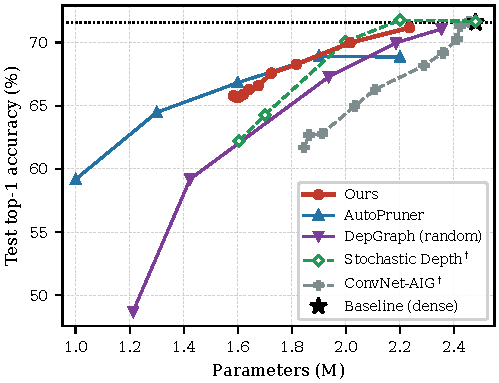
\includegraphics[width=\columnwidth]{figures/mobilenetv2_tinyimagenet200_tradeoff.pdf}
\caption{Test accuracy versus number of parameters of pruned
MobileNetV2 on TinyImageNet-200. Each line connects the models
of one run of our method (one point per pruning cycle) or of one
hyperparameter sweep of a compared method. The star and the
dotted line mark the dense Baseline. $\dagger$: expected number
of executed parameters; these methods store all 2.48M
parameters.}
\Description{Line plot of test top-1 accuracy against the
number of parameters for our method, AutoPruner, DepGraph, Stochastic Depth,
ConvNet-AIG and the dense baseline.}
\label{fig:mbv2-tin-tradeoff}
\end{figure}

%%% Таблица сгенерирована из тех же данных; точность округлена до 0.1
%%% (у AutoPruner в CSV два знака: 59.19, 64.49, 66.83, 68.92, 68.87).
\begin{table}[!t]
\caption{MobileNetV2 on TinyImageNet-200.}
\label{tab:mbv2-tin-all}
\raggedright
\footnotesize
\setlength{\tabcolsep}{2pt}
\renewcommand{\arraystretch}{0.90}
\par\smallskip\noindent\textbf{(a) Pruning trajectory}\par\smallskip
\begin{tabular*}{\columnwidth}{@{\extracolsep{\fill}}lrrrr@{}}
\toprule
\multicolumn{5}{@{}l}{\textbf{Baseline}} \\
\multicolumn{1}{c}{\textbf{Model}} & \multicolumn{1}{c}{\textbf{Params}} & \multicolumn{1}{c}{\textbf{Params}} & \multicolumn{1}{c}{\textbf{Test acc.}} & \multicolumn{1}{c}{\textbf{Acc. change}} \\
\multicolumn{1}{c}{\textbf{}} & \multicolumn{1}{c}{\textbf{(M)}} & \multicolumn{1}{c}{\textbf{(\% of dense)}} & \multicolumn{1}{c}{\textbf{(\%)}} & \multicolumn{1}{c}{\textbf{(pp)}} \\
\textit{dense} & \textit{2.480} & \textit{100.0} & 71.6 & \textit{0.0} \\
\midrule
\multicolumn{5}{@{}l}{\textbf{Ours}} \\
\multicolumn{1}{c}{\textbf{Pruning}} & \multicolumn{1}{c}{\textbf{Params}} & \multicolumn{1}{c}{\textbf{Params}} & \multicolumn{1}{c}{\textbf{Test acc.}} & \multicolumn{1}{c}{\textbf{Acc. change}} \\
\multicolumn{1}{c}{\textbf{cycle}} & \multicolumn{1}{c}{\textbf{(M)}} & \multicolumn{1}{c}{\textbf{(\% of dense)}} & \multicolumn{1}{c}{\textbf{(\%)}} & \multicolumn{1}{c}{\textbf{(pp)}} \\
\textit{1} & \textit{2.235} & \textit{90.1} & 71.2 & \textit{$-$0.4} \\
\textit{2} & \textit{2.015} & \textit{81.3} & 70.0 & \textit{$-$1.6} \\
\textit{3} & \textit{1.817} & \textit{73.3} & 68.3 & \textit{$-$3.3} \\
\textit{4} & \textit{1.725} & \textit{69.5} & 67.6 & \textit{$-$4.0} \\
\textit{5} & \textit{1.676} & \textit{67.6} & 66.6 & \textit{$-$5.0} \\
\textit{6} & \textit{1.642} & \textit{66.2} & 66.3 & \textit{$-$5.3} \\
\textit{7} & \textit{1.620} & \textit{65.3} & 65.9 & \textit{$-$5.7} \\
\textit{8} & \textit{1.605} & \textit{64.7} & 65.7 & \textit{$-$5.9} \\
\textit{9} & \textit{1.593} & \textit{64.2} & 65.7 & \textit{$-$5.9} \\
\textit{10 (final)} & \textit{1.584} & \textit{63.8} & \textbf{65.8} & \textit{$-$5.8} \\
\bottomrule
\end{tabular*}
\par\smallskip\noindent\textbf{(b) Comparison at similar model sizes}\par\smallskip
\setlength{\tabcolsep}{1.2pt}
\begin{tabular*}{\columnwidth}{@{\extracolsep{\fill}}lrrrrrr@{}}
\toprule
\textbf{Size (M)} & \multicolumn{2}{c}{\textbf{Ours}} & \multicolumn{2}{c}{\textbf{AutoPruner}} & \multicolumn{2}{c}{\textbf{DepGraph}} \\
\cmidrule(lr){2-3}\cmidrule(lr){4-5}\cmidrule(lr){6-7}
\multicolumn{1}{c}{\textbf{}} & \multicolumn{1}{c}{\textbf{Acc. (\%)}} & \multicolumn{1}{c}{\textbf{Size (M)}} & \multicolumn{1}{c}{\textbf{Acc. (\%)}} & \multicolumn{1}{c}{\textbf{Size (M)}} & \multicolumn{1}{c}{\textbf{Acc. (\%)}} & \multicolumn{1}{c}{\textbf{Size (M)}} \\
\midrule
\textit{$\approx$1.6} & 65.7 & \textit{1.605} & 66.8 & \textit{1.599} & -- & -- \\
 & \multicolumn{2}{c}{\textit{cycle 8}} & \multicolumn{2}{c}{\textit{r=0.5125}} & \multicolumn{2}{c}{} \\
\midrule
\textit{$\approx$1.9} & 68.3 & \textit{1.817} & 68.9 & \textit{1.900} & 67.3 & \textit{1.936} \\
 & \multicolumn{2}{c}{\textit{cycle 3}} & \multicolumn{2}{c}{\textit{r=0.6792}} & \multicolumn{2}{c}{\textit{$\times$1.25}} \\
\midrule
\textit{$\approx$2.0} & 70.0 & \textit{2.015} & 68.9 & \textit{1.900} & 67.3 & \textit{1.936} \\
 & \multicolumn{2}{c}{\textit{cycle 2}} & \multicolumn{2}{c}{\textit{r=0.6792}} & \multicolumn{2}{c}{\textit{$\times$1.25}} \\
\midrule
\textit{$\approx$2.2} & 71.2 & \textit{2.235} & 68.9 & \textit{2.200} & 70.0 & \textit{2.185} \\
 & \multicolumn{2}{c}{\textit{cycle 1}} & \multicolumn{2}{c}{\textit{r=0.8452}} & \multicolumn{2}{c}{\textit{$\times$1.1}} \\
\bottomrule
\end{tabular*}
\setlength{\tabcolsep}{2pt}
\par\smallskip\noindent Cells (b,c): accuracy (\%); \textit{params (M), setting}.
\par\smallskip\noindent Nearest size within $\pm5\%$; no interpolation. Repeated entries reuse a model. $r$: target channel keep ratio; $\times$: target FLOPs speedup.
\par\smallskip\noindent\textbf{(c) Active-count results\,$\dagger$}\par\smallskip
\begin{tabular*}{\columnwidth}{@{\extracolsep{\fill}}lcccc@{}}
\toprule
\textbf{Method} & $\approx1.6$M & $\approx1.9$M & $\approx2.0$M & $\approx2.2$M \\
\midrule
Stoch. Depth & 62.2 & -- & 70.1 & 71.8 \\
 & \textit{(1.605)} &  & \textit{(2.000)} & \textit{(2.200)} \\
 & \textit{$p_L$=0.000} &  & \textit{$p_L$=0.451} & \textit{$p_L$=0.680} \\
\midrule
ConvNet-AIG & -- & 62.8 & 65.0 & 68.2 \\
 &  & \textit{(1.913)} & \textit{(2.033)} & \textit{(2.289)} \\
 &  & \textit{t=0.1} & \textit{t=0.2} & \textit{t=0.4} \\
\bottomrule
\end{tabular*}
\par\smallskip\noindent $\dagger$: both store 2.48M parameters. AIG reports test means; SD reports expected active counts under sampled test masks. Active counts are not storage or latency measurements.
\par\smallskip\noindent One run per setting; the ten Ours points share one run. Training budgets differ.
\par\smallskip\noindent In (a), shares and changes use the dense Baseline (2{,}480{,}072 parameters); pp denotes percentage points.
\par\smallskip\noindent Full sweeps: Table~\ref{tab:mbv2-tin-full}.
\end{table}

\paragraph{Iterative channel pruning.}
Figure~\ref{fig:mbv2-tin-tradeoff} and
Table~\ref{tab:mbv2-tin-all} show the accuracy--size trade-off
of all methods. The dense Baseline reaches 71.6\% accuracy
with 2.48M parameters.

\emph{Mild compression.} The first two cycles of our method
remove 9.9\% and 18.7\% of the parameters, with accuracy
losses of 0.4 and 1.6 percentage points, respectively.
At 2.015M parameters, our model reaches 70.0\% accuracy,
matching DepGraph at 2.185M. The closest AutoPruner model
by parameter count reaches 68.9\% at 1.900M.

Stochastic Depth reaches 71.8\% at a reported expected active count
of 2.2M under sampled test masks. ConvNet-AIG stays
within 0.3 percentage points of the Baseline for $t\geq0.7$,
with test-mean active counts of 97.7--99.2\% of its parameters.
Both retain all 2.48M parameters in storage.

\emph{Stronger compression.} Our final model reaches 65.8\%
accuracy at 1.584M parameters. AutoPruner is more accurate
at a similar size, reaching 66.8\% at 1.599M.
Below 1.5M parameters in Figure~\ref{fig:mbv2-tin-tradeoff},
only AutoPruner and DepGraph provide comparison points.
 AutoPruner gives the strongest observed
accuracy--size trade-off in this range, reaching 64.5\%
at 1.300M, compared with DepGraph's 59.2\% at 1.423M.
%%% <<< END [MBV2-TIN] <<<

\paragraph{Single-pass channel pruning.}
The seven one-iteration MobileNetV2 models in
Figure~\ref{fig:additional-pruning-trajectories}(a) and
Table~\ref{tab:mbv2-one-iteration} span 1.262--2.235M
parameters and 60.7--71.1\% reported test accuracy. At nearly the
same size, the one-iteration model reaches 69.5\% at 2.013M,
compared with 70.0\% at 2.015M on the existing iterative
trajectory; at 1.813M it reaches 68.4\%, compared with 68.3\%
at 1.817M. These observations do not show a consistent advantage
for either procedure.

\subsubsection{ResNet-50 on CIFAR-10}

%%% >>> BEGIN [RN50-C10] >>>
% Existing one-shot/comparator measurements are retained at table precision in
% ../data/manuscript_comparators.csv; new trajectories: ../data/graphics_results.csv.
\begin{figure*}[t]
  \centering
  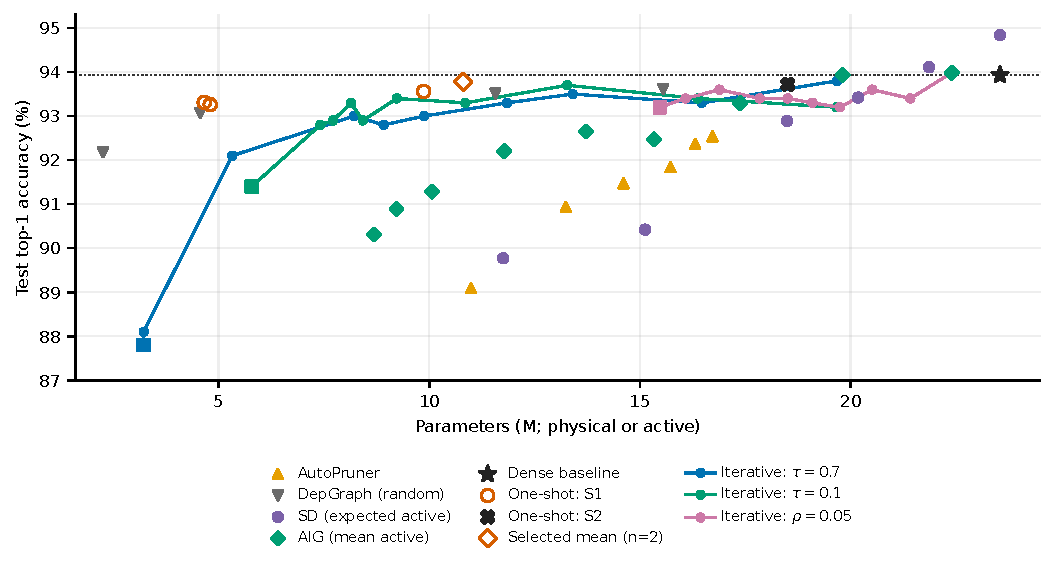
\includegraphics[width=\textwidth]{figures/resnet50_cifar10_selected.pdf}
  \caption{ResNet-50 on CIFAR-10. Fixed networks: the existing one-shot
    results, all 30 iterative channel-pruning models, AutoPruner and
    DepGraph (random importance). Lines follow cycle order and squares
    mark final iterative models. The hollow diamond is a coordinate-wise
    mean of two selected same-seed runs out of eight; it is not a deployed
    network. Dynamic baselines retain the full backbone: AIG counts
    are validation means and SD counts are expectations. Training budgets
    and historical accuracy aggregation differ.}
  \label{fig:resnet-cifar-tradeoff}
  \Description{One plot compares three iterative ResNet channel-pruning
    trajectories, the one-shot models, structural-pruning comparators and
    dynamic baselines, using physical or active parameter counts.}
\end{figure*}

\paragraph{One-shot pruning.}
Figure~\ref{fig:resnet-cifar-tradeoff} and Table~\ref{tab:resnet-cifar-all}
show the trade-off between accuracy and model size for ResNet-50 on
CIFAR-10. The dense
baseline achieves 93.93\% test accuracy with 23.547M parameters.

Our 4.660M-parameter model achieves 93.31\% accuracy, reducing the
parameter count by 80.2\% with an accuracy loss of 0.62 percentage points.
The nearest DepGraph model achieves 93.07\% with 4.566M parameters.
Our model therefore achieves 0.24 percentage points higher accuracy
with 2.1\% more parameters.

Averaging two selected repeats gives 10.805M parameters and
93.78\% accuracy, corresponding to 54.1\% fewer parameters and an
accuracy gap of 0.15 percentage points from the dense baseline.
The nearest DepGraph model achieves 93.51\% with 11.569M parameters.

Stochastic Depth reaches up to 94.84\% accuracy but retains all
23.547M parameters in storage.

\paragraph{Iterative channel pruning.}
Three channel-pruning trajectories in
Figure~\ref{fig:resnet-cifar-tradeoff} contain ten
models each, ordered by cycle rather than by notebook row order.
The threshold series $\tau=0.7$ reaches 92.1\% at 5.325M
parameters before declining to 87.8\% at 3.220M in its final
model. The $\tau=0.1$ series ends at 91.4\% with 5.787M
parameters. The budget-only series $\rho=0.05$ retains 15.475M parameters with
93.2\% accuracy at the end. Complete trajectories are given in
Table~\ref{tab:resnet-notebook-trajectories}.

\paragraph{Block pruning.}
Four historical block-pruning models in Figure~\ref{fig:additional-pruning-trajectories}(b) span 15.266--18.974M parameters and 92.80--93.27\%
reported accuracy. Their final and preceding recovery models
have the same parameter count but different accuracies;
they are separate checkpoints, not seed repetitions.

% Existing rows retain their previously reported precision and accuracy changes.
% Generated by paper/scripts/build_results.py from graphics_results.csv.

\newcommand{\ResNetIterativeFinalRows}{%
$\tau=0.7$ & 3.220 & 13.7 & 87.8 & -6.13 \\
$\tau=0.1$ & 5.787 & 24.6 & 91.4 & -2.53 \\
$\rho=0.05$ & 15.475 & 65.7 & 93.2 & -0.73 \\
}

\begin{table*}[t]
  \caption{ResNet-50/CIFAR-10 one-shot and comparator results, with the three
    final iterative channel-pruning models. All 30 iterative checkpoints
    are listed in Table~\ref{tab:resnet-notebook-trajectories}. Params: reported parameter
    count (M) and its share of the dense model (23{,}547{,}338 parameters,
    \%). $\Delta$: accuracy difference from the Baseline in percentage
    points. S1 and S2 denote our two sweeps; the following pair gives
    $\delta_s/\delta_h$ in percentage points. Mean averages both
    coordinates of two selected runs from eight same-configuration,
    same-seed repeats; it is not one deployed network.
    Iterative settings use threshold $\tau$ or budget fraction $\rho$.
    DepGraph settings are target FLOPs speedups; $k$ is AutoPruner's
    target keep ratio, $p_L$ the final survival probability, and $t$
    the ConvNet-AIG target rate. $\dagger$: expected active parameters
    under stochastic inference; $\ddagger$: active parameters averaged
    over validation images. Both marked methods retain the full backbone
    weights. Training budgets and historical accuracy aggregation differ.}
  \label{tab:resnet-cifar-all}
  \centering
  \small
  \setlength{\tabcolsep}{4pt}
  \begin{minipage}[t]{0.48\textwidth}
    \centering
    \begin{tabular}[t]{@{}lrrrr@{}}
      \toprule
      Setting & Params (M) & \% & Acc. (\%) & $\Delta$ \\
      \midrule
      \multicolumn{5}{l}{\textit{Baseline}} \\
      % 716de1ac4ae743689a7962a3a4dfae3b
      dense & 23.547 & 100.0 & 93.93 & 0.00 \\
      \midrule
      \multicolumn{5}{l}{\textit{Ours: one-shot (selected)}} \\
      % resnet50_cifar10_ls0_curve7_v1/large_18m
      S1: $0.025/0.05$ & 4.660 & 19.8 & 93.31 & $-$0.62 \\
      % resnet50_cifar10_ls0_curve7_v1/middle_8m
      S1: $0.25/0.5$ & 4.801 & 20.4 & 93.26 & $-$0.67 \\
      % resnet50_cifar10_ls0_curve7_v1/floor_probe_2p9m
      S1: $5/10$ & 9.868 & 41.9 & 93.56 & $-$0.37 \\
      % resnet50_cifar10_ls0_prebn_repeat8_v1/mean_selected_repeats_05_07
      Mean ($n=2$) & 10.805 & 45.9 & 93.78 & $-$0.15 \\
      % resnet50_cifar10_ls0_curve7_v2/middle_8m
      S2: $0.25/0.5$ & 18.512 & 78.6 & 93.72 & $-$0.21 \\
      \midrule
      \multicolumn{5}{l}{\textit{Ours: iterative (final cycle)}} \\
      \ResNetIterativeFinalRows
      \midrule
      \multicolumn{5}{l}{\textit{DepGraph (random importance)}} \\
      % a66ef23af1d94813bf2629ffec935f40
      $\times1.5$ & 15.554 & 66.1 & 93.62 & $-$0.31 \\
      % ab961d162f4646cb8773ab9f7445607f
      $\times2.0$ & 11.569 & 49.1 & 93.51 & $-$0.42 \\
      % 60622bbe09914eb8aa7a2b0906acf673
      $\times5.0$ & 4.566 & 19.4 & 93.07 & $-$0.86 \\
      % 6839c67c7d974f949927e1deafd78957
      $\times10.0$ & 2.258 & 9.6 & 92.18 & $-$1.75 \\
      \midrule
      \multicolumn{5}{l}{\textit{AutoPruner}} \\
      % AutoPruner keep=0.3
      $k=0.3$ & 10.993 & 46.7 & 89.09 & $-$4.84 \\
      % AutoPruner keep=0.5
      $k=0.5$ & 13.242 & 56.2 & 90.94 & $-$2.99 \\
      % AutoPruner keep=0.6
      $k=0.6$ & 14.612 & 62.1 & 91.47 & $-$2.45 \\
      % AutoPruner keep=0.7
      $k=0.7$ & 15.728 & 66.8 & 91.84 & $-$2.09 \\
      % AutoPruner keep=0.8
      $k=0.8$ & 16.312 & 69.3 & 92.37 & $-$1.55 \\
      % AutoPruner keep=0.9
      $k=0.9$ & 16.722 & 71.0 & 92.54 & $-$1.39 \\
      \bottomrule
    \end{tabular}
  \end{minipage}\hfill
  \begin{minipage}[t]{0.48\textwidth}
    \centering
    \begin{tabular}[t]{@{}lrrrr@{}}
      \toprule
      Setting & Params (M) & \% & Acc. (\%) & $\Delta$ \\
      \midrule
      \multicolumn{5}{l}{\textit{Stochastic Depth}} \\
      % Stochastic Depth p_L=0.3
      $p_L=0.3$ & 11.756$^\dagger$ & 49.9 & 89.77 & $-$4.16 \\
      % Stochastic Depth p_L=0.5
      $p_L=0.5$ & 15.125$^\dagger$ & 64.2 & 90.42 & $-$3.50 \\
      % Stochastic Depth p_L=0.7
      $p_L=0.7$ & 18.494$^\dagger$ & 78.5 & 92.89 & $-$1.04 \\
      % Stochastic Depth p_L=0.8
      $p_L=0.8$ & 20.179$^\dagger$ & 85.7 & 93.42 & $-$0.51 \\
      % Stochastic Depth p_L=0.9
      $p_L=0.9$ & 21.863$^\dagger$ & 92.8 & 94.11 & $+$0.18 \\
      % Stochastic Depth p_L=1.0
      $p_L=1.0$ & 23.547$^\dagger$ & 100.0 & 94.84 & $+$0.91 \\
      \midrule
      \multicolumn{5}{l}{\textit{ConvNet-AIG}} \\
      % bffb9a169ea949aeb7f6853eb49272f7
      $t=0.1$ & 8.696$^\ddagger$ & 36.9 & 90.31 & $-$3.62 \\
      % 9512a6073f7e41a5adb6758211a6a555
      $t=0.2$ & 9.224$^\ddagger$ & 39.2 & 90.88 & $-$3.05 \\
      % b6b35731d7f74cd8b9ffd790c8b71864
      $t=0.3$ & 10.068$^\ddagger$ & 42.8 & 91.28 & $-$2.65 \\
      % a447cf7d416e49d9a145881241071636
      $t=0.4$ & 11.783$^\ddagger$ & 50.0 & 92.20 & $-$1.73 \\
      % 85ef57c9020e449e83d9b9939fa9d50c
      $t=0.5$ & 13.717$^\ddagger$ & 58.3 & 92.65 & $-$1.28 \\
      % eb38db75adaa43658ba861536699ccc5
      $t=0.6$ & 15.335$^\ddagger$ & 65.1 & 92.47 & $-$1.45 \\
      % 5f97b677390845d7995d4c3f904ee954
      $t=0.7$ & 17.383$^\ddagger$ & 73.8 & 93.29 & $-$0.64 \\
      % 500f50a024014ba4bf57ec7b92d91931
      $t=0.8$ & 19.811$^\ddagger$ & 84.1 & 93.93 & 0.00 \\
      % 1664739e725b4bf0ae0bf87df187ee91
      $t=0.9$ & 22.406$^\ddagger$ & 95.2 & 93.98 & $+$0.05 \\
      \bottomrule
    \end{tabular}
  \end{minipage}
\end{table*}

%%% <<< END [RN50-C10] <<<

% Additional historical results from actual graphics (2).ipynb, 2026-11-07.
% Exact values and per-row provenance: ../new_points.csv.
\begin{figure*}[t]
  \centering
  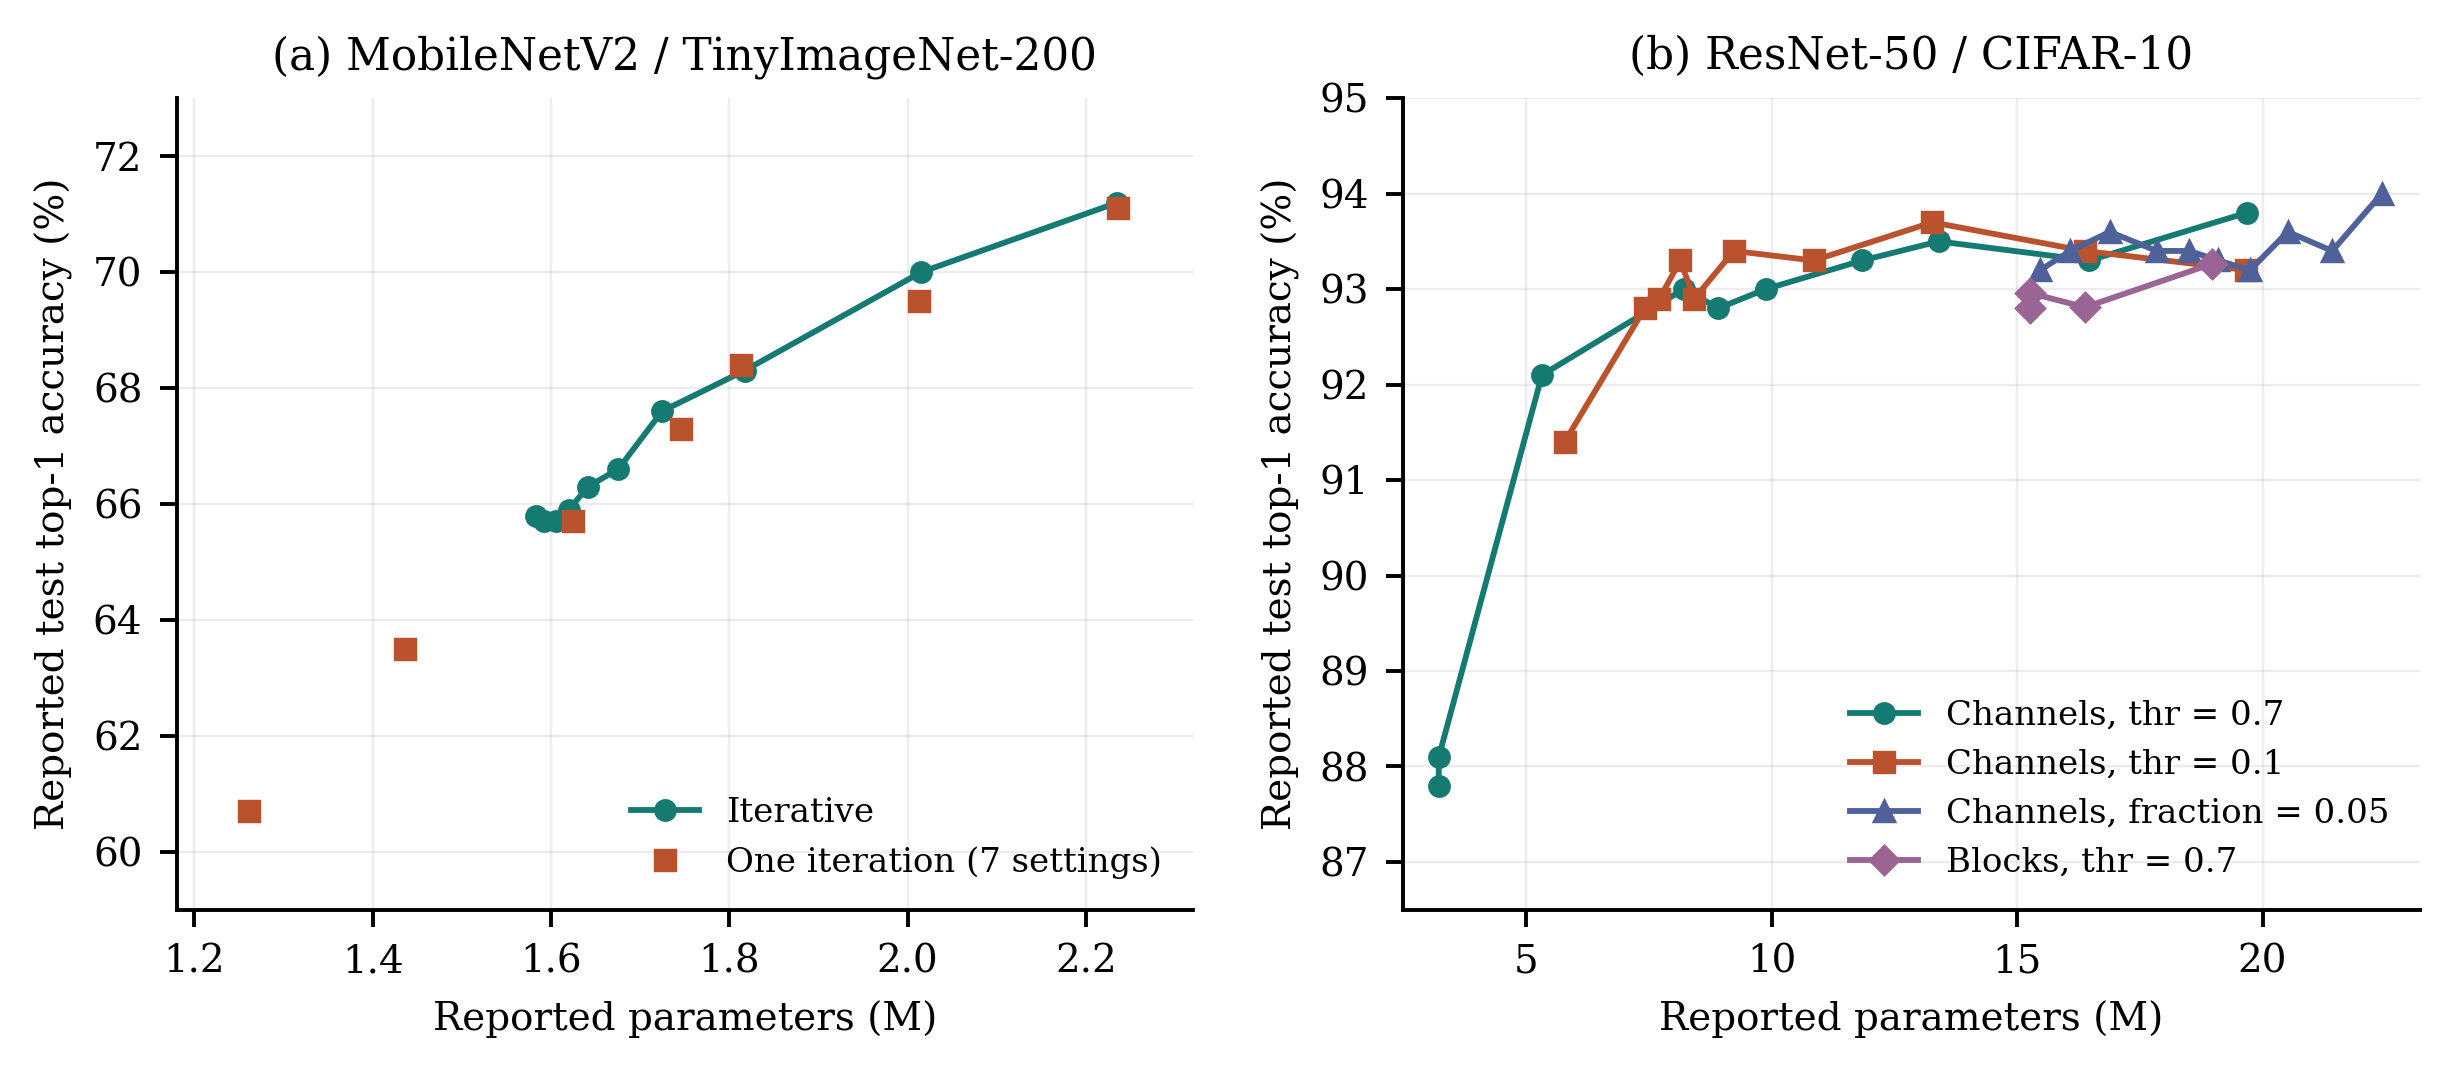
\includegraphics[width=\textwidth]{figures/additional_pruning_trajectories.png}
  \caption{Additional notebook-reported pruning results.
    (a) Seven one-iteration MobileNetV2 settings and the existing
    iterative trajectory. (b) Three iterative channel-pruning
    trajectories and one block-pruning trajectory for ResNet-50.
    Lines connect successive recorded cycles; the final model is
    placed last. Squares in (a) are separate settings, not cycles.
    Counts are reported model parameters, not FLOPs or active-count
    estimates. No uncertainty bars or matched-budget claim are implied.}
  \Description{Two panels of reported test accuracy against model
    parameters. MobileNetV2 compares seven one-iteration settings
    with ten iterative models. ResNet-50 shows thirty channel-pruning
    models in three trajectories and four block-pruning models.}
  \label{fig:additional-pruning-trajectories}
\end{figure*}


\subsection{Computational Efficiency}
\subsection{Effect of Adaptive \texorpdfstring{$\lambda$}{lambda} Scheduling}
\subsection{Iterative Pruning Analysis}

%%% >>> BEGIN [MBV2-TIN] MobileNetV2 + TinyImageNet-200 >>>
\paragraph{MobileNetV2 on TinyImageNet-200.}
Our run yields one model per cycle
(Table~\ref{tab:mbv2-tin-all}). Most parameters are removed in
the first cycles: after three cycles it has removed 26.7\% of the dense
parameters. Between cycle~5 and the final model the size
changes only from 67.6\% to 63.8\% of the dense model
(accuracy from 66.6\% to 65.8\%). These are single-run observations.
%%% <<< END [MBV2-TIN] <<<

\subsection{Ablation Studies}
% Retained method diagnostics from the previous manuscript: E1, E5, E6.
\label{sec:ablation-studies}

We report three diagnostic studies on ResNet-50/CIFAR-10.
Test accuracies are measured on the official test set after
validation-based checkpoint selection. The comparisons are exploratory:
their outcomes informed subsequent experiments. Each comparison has
its own architecture and training protocol, as specified below.
Figure~\ref{fig:resnet-cifar-ablations} summarizes these studies.

\begin{figure*}[t]
  \centering
  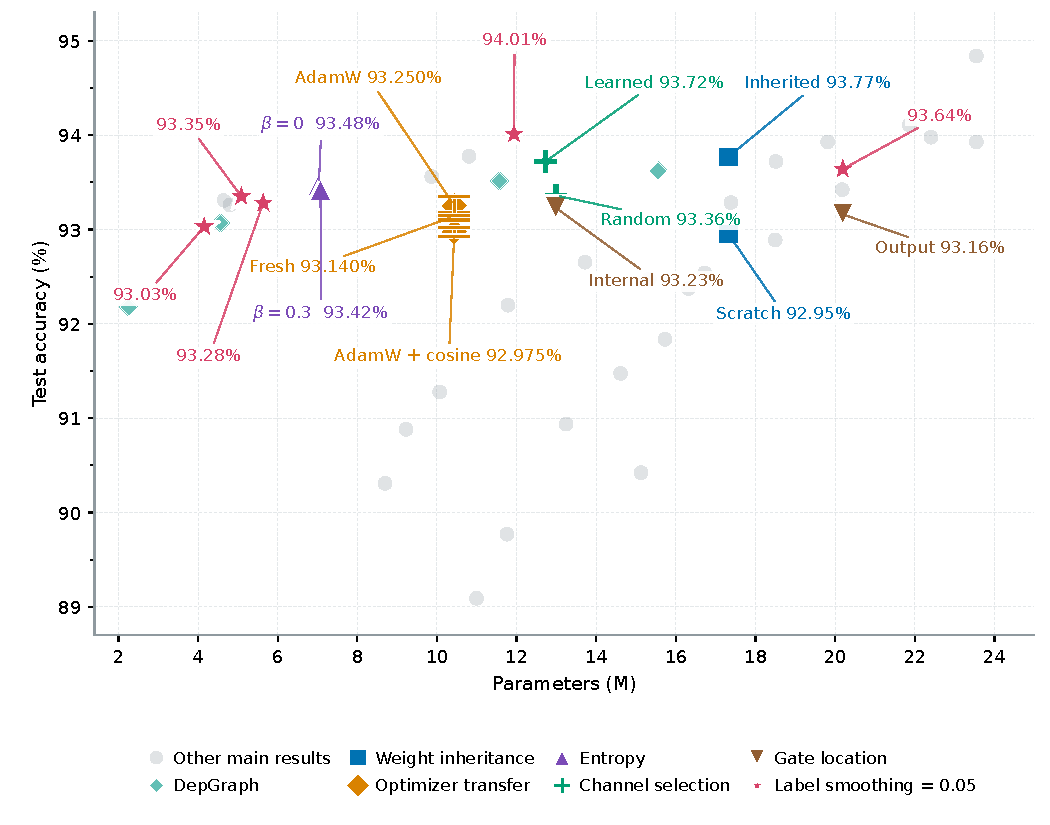
\includegraphics[width=\textwidth]{figures/resnet50_cifar10_ablations.pdf}
  \caption{Three ResNet-50/CIFAR-10 diagnostics. Labels give physical
    parameter counts. Only the weight-initialization pair fixes the
    architecture and search checkpoint; selection and gate-placement
    comparisons use different architectures or training protocols.}
  \label{fig:resnet-cifar-ablations}
  \Description{Three panels compare inherited and random weights,
    adaptive and historical random selection recipes, and internal and
    output gates. No uncertainty intervals are implied.}
\end{figure*}


% E1
\paragraph{Weight inheritance.}
We fix a pruned architecture with 17{,}321{,}706 parameters and
compare inherited and randomly initialized weights. Both branches
use the same 60-epoch search result followed by 90 epochs of recovery.
Inherited weights reach 93.77\% test accuracy, compared with
92.95\% from random initialization, a difference of
0.82 percentage points (Table~\ref{tab:ablation-weights}).
This result concerns one selected architecture and one search result;
it does not establish an advantage across architectures or training seeds.

\begin{table}[t]
  \centering
  \caption{Recovery initialization for a fixed architecture.
    Accuracy is reported in percent.}
  \label{tab:ablation-weights}
  \begin{tabular}{@{}lrr@{}}
    \toprule
    Initialization & Validation & Test \\
    \midrule
    Inherited weights & 94.38 & 93.77 \\
    Random weights & 93.82 & 92.95 \\
    \bottomrule
  \end{tabular}
\end{table}
% E2
% \paragraph{Optimizer and scheduler state transfer.}
% For a separate, fixed 10{,}435{,}943-parameter architecture, we compare
% three recovery policies from a common search checkpoint, with a
% 60/90 search/recovery split and two recovery repetitions per policy.
% With a restarted cosine schedule, transferring AdamW states gives
% 93.250\% mean test accuracy, compared with 93.140\% using fresh
% states (Table~\ref{tab:ablation-optimizer}). This 0.11-point difference
% changes sign between repetitions. Continuing the cosine schedule
% with transferred AdamW states gives 92.975\%, 0.275 points below
% restarting it. Two recovery repetitions do not support a strong
% statistical conclusion.

% \begin{table}[t]
%   \centering
%   \caption{Test accuracy (\%) for state-transfer policies.
%     The mean is computed over the two recovery repetitions.}
%   \label{tab:ablation-optimizer}
%   \small
%   \setlength{\tabcolsep}{3pt}
%   \begin{tabular}{@{}llrrr@{}}
%     \toprule
%     AdamW & Cosine & Rep.~1 & Rep.~2 & Mean \\
%     \midrule
%     Fresh & Restarted & 93.18 & 93.10 & 93.140 \\
%     Transferred & Restarted & 93.15 & 93.35 & 93.250 \\
%     Transferred & Continued & 92.93 & 93.02 & 92.975 \\
%     \bottomrule
%   \end{tabular}
% \end{table}
% % E4
% \paragraph{Entropy regularization at similar sizes.}
% We compare two runs with $\beta=0$ and $\beta=0.3$, retrospectively
% selected for their similar physical parameter counts. Both use
% 60 epochs of search, 90 epochs of recovery, adaptive $\lambda$,
% and the same accuracy tolerances and selector based on the expected
% open count.
% The $\beta=0$ model reaches 93.48\% test accuracy at 7.034M
% parameters; the $\beta=0.3$ model reaches 93.42\% at 7.073M
% (Table~\ref{tab:ablation-entropy}). The observed difference is
% 0.06 percentage points. These single-seed runs come from different
% series and code revisions and have different architectures and MAC
% counts, so the pair does not isolate the effect of entropy regularization.

% \begin{table}[t]
%   \centering
%   \caption{Entropy comparison using physical deployment sizes.
%     Accuracy is in percent; M and G denote millions and billions.}
%   \label{tab:ablation-entropy}
%   \small
%   \setlength{\tabcolsep}{4pt}
%   \begin{tabular}{@{}rrrrr@{}}
%     \toprule
%     $\beta$ & Params (M) & MACs (G) & Validation & Test \\
%     \midrule
%     0 & 7.034 & 0.538 & 93.92 & 93.48 \\
%     0.3 & 7.073 & 0.503 & 93.96 & 93.42 \\
%     \bottomrule
%   \end{tabular}
% \end{table}
% E5
\paragraph{Comparison with random channel selection.}
A separate later adaptive run reaches 93.72\% test accuracy with
12.728M parameters, compared with 93.36\% at 12.984M for a
historical random-selection control (Table~\ref{tab:ablation-random}).
Both models use 150 training epochs, but the adaptive run uses a
single 60-epoch search followed by 90 epochs of recovery, whereas
the random control uses an earlier iterative protocol with fixed
$\lambda$. The random model also has fewer MACs: 0.692G versus
1.108G. The 0.36-point accuracy difference therefore compares
complete training recipes and does not isolate channel ranking
or adaptive sparsity scheduling.

\begin{table}[t]
  \centering
  \caption{Historical random control and the later adaptive recipe.
    Sizes describe physical models; test accuracy is in percent.}
  \label{tab:ablation-random}
  \small
  \setlength{\tabcolsep}{4pt}
  \begin{tabular}{@{}lrrr@{}}
    \toprule
    Method & Params (M) & MACs (G) & Test \\
    \midrule
    Random selection & 12.984 & 0.692 & 93.36 \\
    Our adaptive recipe & 12.728 & 1.108 & 93.72 \\
    \bottomrule
  \end{tabular}
\end{table}
% E6
\paragraph{Internal and output channel gates.}
An earlier experiment uses fixed $\lambda=0.001$ and 150 training
epochs per model to compare gates on residual-branch outputs with
gates on internal bottleneck channels. Internal gating produces
12.983M parameters at 93.23\% test accuracy, compared with
20.189M at 93.16\% for output gating
(Table~\ref{tab:ablation-gate-location}). These runs demonstrate
a smaller model at similar accuracy, but their pruning budgets
and resulting architectures differ. They do not isolate gate
placement at a fixed size or evaluate adaptive scheduling.

\begin{table}[t]
  \centering
  \caption{Gate placement in the early fixed-$\lambda$ experiment.
    Accuracy is in percent and parameter counts are physical.}
  \label{tab:ablation-gate-location}
  \begin{tabular}{@{}lrrr@{}}
    \toprule
    Gate location & Params (M) & Validation & Test \\
    \midrule
    Branch output & 20.189 & 93.88 & 93.16 \\
    Bottleneck internal & 12.983 & 94.04 & 93.23 \\
    \bottomrule
  \end{tabular}
\end{table}

% E8: historical label-smoothed recovery; red stars in the working notebook.
% \paragraph{Label smoothing during recovery.}
% We additionally report five historical runs with label smoothing
% $\varepsilon_{\mathrm{LS}}=0.05$ during recovery
% (Table~\ref{tab:ablation-label-smoothing}). Search uses ordinary
% cross-entropy without label smoothing. Each run uses 60 epochs
% of adaptive mask search followed by 90 epochs of recovery,
% with seed~42, a minimum channel-retention ratio of 0.08 and
% entropy regularization disabled. The five runs use different
% accuracy tolerances and produce different pruned architectures.
% Among these five runs, the highest test accuracy is
% \textbf{94.01\%} with \textbf{11.934M} parameters; a smaller model reaches 93.35\%
% with 5.086M parameters.

% The search learning-rate floor is $6.6443\cdot10^{-4}$,
% compared with zero in the main series; there is also no
% separate BatchNorm recalibration before recovery.
% The results therefore characterize the complete training recipe;
% they do not isolate the effect of label smoothing alone.

% \begin{table}[t]
%   \centering
%   \caption{Historical runs with label smoothing 0.05 during
%     recovery. Parameter counts are physical; accuracy is measured
%     on the official CIFAR-10 test set.}
%   \label{tab:ablation-label-smoothing}
%   \begin{tabular}{@{}rr@{}}
%     \toprule
%     Parameters (M) & Test accuracy (\%) \\
%     \midrule
%     4.154 & 93.03 \\
%     5.086 & 93.35 \\
%     5.637 & 93.28 \\
%     \textbf{11.934} & \textbf{94.01} \\
%     20.192 & 93.64 \\
%     \bottomrule
%   \end{tabular}
% \end{table}
% % Points: notebooks/data/selected_parameter_curve_red_stars.csv, Ours (selected).
% % Test sources: user frozen-test report 2026-09-23 for the first three;
% % parameter_curve_target13m_17m_results.tar.gz/test_comparison.csv for the last two.
% % Actual phase configs: parameter_curve_4x150_results.tar.gz and the 13m/17m archive.
% % For approx9m_retry, recovery LS=.05 is reconstructed from its launch command
% % and parameter_curve_recovery90_ls005; the effective retry config was not retained.
% % Source audit: tasks/adhoc/pruning-accuracy-parameters-plot/
% % selected-red-star-runs.md and ours-selected-configuration-comparison.md.


\section{Discussion}
\subsection{Limitations}
\subsection{Future Work}

\section{Conclusion}
Conclusion text.

%%
%% Acknowledgments
%%
\begin{acks}
Acknowledgments text.
\end{acks}

%%
%% Bibliography
%%
%%% >>> BEGIN [MBV2-TIN] MobileNetV2 + TinyImageNet-200 >>>
%%% Записи для ключей \cite из этой части находятся в sample-base.bib:
%%% le2015tiny — Y. Le, X. Yang. Tiny ImageNet Visual Recognition Challenge, 2015.
%%% sandler2018mobilenetv2 — M. Sandler et al. MobileNetV2: Inverted Residuals and Linear Bottlenecks. CVPR 2018.
%%% fang2023depgraph — G. Fang et al. DepGraph: Towards Any Structural Pruning. CVPR 2023.
%%% luo2020autopruner — J.-H. Luo, J. Wu. AutoPruner: An End-to-End Trainable Filter Pruning Method
%%% for Efficient Deep Model Inference. Pattern Recognition, 2020.
%%% veit2018convnet — A. Veit, S. Belongie. Convolutional Networks with Adaptive Inference Graphs.
%%% ECCV 2018 (журнальная версия: IJCV 2020).
%%% huang2016deep — G. Huang et al. Deep Networks with Stochastic Depth. ECCV 2016.
%%% <<< END [MBV2-TIN] <<<
\bibliographystyle{ACM-Reference-Format}
\bibliography{sample-base}

%%
%% Appendices
%%
\appendix

\section{Additional Experiments}
\subsection{Detailed Results}

Table~\ref{tab:mbv2-tin-full} retains all MobileNetV2 settings and
results underlying Figure~\ref{fig:mbv2-tin-tradeoff};
Table~\ref{tab:mbv2-tin-all} highlights comparisons at similar sizes.

\begin{table}[!t]
\caption{Complete MobileNetV2 results on TinyImageNet-200. Shares and accuracy changes
are relative to the dense Baseline (2{,}480{,}072 parameters);
pp denotes percentage points. $\dagger$: test-mean active parameters
for ConvNet-AIG; analytical expected active parameters for Stochastic
Depth. Both store 2.48M parameters; Stochastic Depth skips closed residual
branches at test time.}
\label{tab:mbv2-tin-full}
\centering
\footnotesize
\setlength{\tabcolsep}{2pt}
\renewcommand{\arraystretch}{0.88}
\sisetup{mode=text, reset-text-series=false, retain-explicit-plus=true}
\begin{tabular*}{\columnwidth}{@{\extracolsep{\fill}}l
  S[table-format=1.3] S[table-format=3.1]
  S[table-format=2.1] S[table-format=+2.1]@{}}
\toprule
\multicolumn{5}{@{}l}{\textbf{Baseline}} \\
\textbf{Model} & \multicolumn{1}{c}{\textbf{Params}} & \multicolumn{1}{c}{\textbf{Params}} & \multicolumn{1}{c}{\textbf{Test acc.}} & \multicolumn{1}{c}{\textbf{Acc. change}} \\
{} & \multicolumn{1}{c}{\textbf{(M)}} & \multicolumn{1}{c}{\textbf{(\% of dense)}} & \multicolumn{1}{c}{\textbf{(\%)}} & \multicolumn{1}{c}{\textbf{(pp)}} \\[1pt]
dense & 2.480 & 100.0 & 71.6 & 0.0 \\
\midrule
\multicolumn{5}{@{}l}{\textbf{Ours}} \\
\textbf{Pruning} & \multicolumn{1}{c}{\textbf{Params}} & \multicolumn{1}{c}{\textbf{Params}} & \multicolumn{1}{c}{\textbf{Test acc.}} & \multicolumn{1}{c}{\textbf{Acc. change}} \\
\textbf{cycle} & \multicolumn{1}{c}{\textbf{(M)}} & \multicolumn{1}{c}{\textbf{(\% of dense)}} & \multicolumn{1}{c}{\textbf{(\%)}} & \multicolumn{1}{c}{\textbf{(pp)}} \\[1pt]
1 & 2.235 & 90.1 & 71.2 & -0.4 \\
2 & 2.015 & 81.3 & 70.0 & -1.6 \\
3 & 1.817 & 73.3 & 68.3 & -3.3 \\
4 & 1.725 & 69.5 & 67.6 & -4.0 \\
5 & 1.676 & 67.6 & 66.6 & -5.0 \\
6 & 1.642 & 66.2 & 66.3 & -5.3 \\
7 & 1.620 & 65.3 & 65.9 & -5.7 \\
8 & 1.605 & 64.7 & 65.7 & -5.9 \\
9 & 1.593 & 64.2 & 65.7 & -5.9 \\
\bfseries 10 (final) & \bfseries 1.584 & \bfseries 63.8 & \bfseries 65.8 & \bfseries -5.8 \\
\midrule
\multicolumn{5}{@{}l}{\textbf{DepGraph (random importance)}} \\
\textbf{Target FLOPs} & \multicolumn{1}{c}{\textbf{Params}} & \multicolumn{1}{c}{\textbf{Params}} & \multicolumn{1}{c}{\textbf{Test acc.}} & \multicolumn{1}{c}{\textbf{Acc. change}} \\
\textbf{speedup} & \multicolumn{1}{c}{\textbf{(M)}} & \multicolumn{1}{c}{\textbf{(\% of dense)}} & \multicolumn{1}{c}{\textbf{(\%)}} & \multicolumn{1}{c}{\textbf{(pp)}} \\[1pt]
$\times1.05$ & 2.354 & 94.9 & 71.1 & -0.5 \\
$\times1.1$ & 2.185 & 88.1 & 70.0 & -1.6 \\
$\times1.25$ & 1.936 & 78.1 & 67.3 & -4.3 \\
$\times1.5$ & 1.423 & 57.4 & 59.2 & -12.4 \\
$\times2.0$ & 1.212 & 48.9 & 48.7 & -22.9 \\
\midrule
\multicolumn{5}{@{}l}{\textbf{AutoPruner}} \\
\textbf{Target channel} & \multicolumn{1}{c}{\textbf{Params}} & \multicolumn{1}{c}{\textbf{Params}} & \multicolumn{1}{c}{\textbf{Test acc.}} & \multicolumn{1}{c}{\textbf{Acc. change}} \\
\textbf{keep ratio} & \multicolumn{1}{c}{\textbf{(M)}} & \multicolumn{1}{c}{\textbf{(\% of dense)}} & \multicolumn{1}{c}{\textbf{(\%)}} & \multicolumn{1}{c}{\textbf{(pp)}} \\[1pt]
0.1809 & 1.000 & 40.3 & 59.2 & -12.4 \\
0.3469 & 1.300 & 52.4 & 64.5 & -7.1 \\
0.5125 & 1.599 & 64.5 & 66.8 & -4.8 \\
0.6792 & 1.900 & 76.6 & 68.9 & -2.7 \\
0.8452 & 2.200 & 88.7 & 68.9 & -2.7 \\
\midrule
\multicolumn{5}{@{}l}{\textbf{Stochastic Depth\,\textsuperscript{$\dagger$}}} \\
\textbf{Survival} & \multicolumn{1}{c}{\textbf{Active params}} & \multicolumn{1}{c}{\textbf{Params}} & \multicolumn{1}{c}{\textbf{Test acc.}} & \multicolumn{1}{c}{\textbf{Acc. change}} \\
\textbf{prob. $p_L$} & \multicolumn{1}{c}{\textbf{(M)}} & \multicolumn{1}{c}{\textbf{(\% of dense)}} & \multicolumn{1}{c}{\textbf{(\%)}} & \multicolumn{1}{c}{\textbf{(pp)}} \\[1pt]
0.000 & 1.605 & 64.7 & 62.2 & -9.4 \\
0.109 & 1.700 & 68.5 & 64.3 & -7.3 \\
0.451 & 2.000 & 80.6 & 70.1 & -1.5 \\
0.680 & 2.200 & 88.7 & 71.8 & +0.2 \\
1.000 & 2.480 & 100.0 & 71.7 & +0.1 \\
\midrule
\multicolumn{5}{@{}l}{\textbf{ConvNet-AIG\,\textsuperscript{$\dagger$}}} \\
\textbf{Target} & \multicolumn{1}{c}{\textbf{Active params}} & \multicolumn{1}{c}{\textbf{Params}} & \multicolumn{1}{c}{\textbf{Test acc.}} & \multicolumn{1}{c}{\textbf{Acc. change}} \\
\textbf{rate $t$} & \multicolumn{1}{c}{\textbf{(M)}} & \multicolumn{1}{c}{\textbf{(\% of dense)}} & \multicolumn{1}{c}{\textbf{(\%)}} & \multicolumn{1}{c}{\textbf{(pp)}} \\[1pt]
0.01 & 1.845 & 74.4 & 61.7 & -9.9 \\
0.05 & 1.864 & 75.1 & 62.7 & -8.9 \\
0.1 & 1.913 & 77.1 & 62.8 & -8.8 \\
0.2 & 2.033 & 82.0 & 65.0 & -6.6 \\
0.3 & 2.108 & 85.0 & 66.3 & -5.3 \\
0.4 & 2.289 & 92.3 & 68.2 & -3.4 \\
0.5 & 2.360 & 95.1 & 69.2 & -2.4 \\
0.6 & 2.411 & 97.2 & 70.3 & -1.3 \\
0.7 & 2.423 & 97.7 & 71.3 & -0.3 \\
0.8 & 2.457 & 99.1 & 71.7 & +0.1 \\
0.9 & 2.459 & 99.2 & 71.6 & 0.0 \\
\bottomrule
\end{tabular*}
\end{table}

% Notebook values: 37 literal rows plus four exact matched-Run-ID rows.
\begin{table}[t]
  \caption{Seven one-iteration MobileNetV2 models from the additional
    notebook. Settings reproduce \texttt{thr}/\texttt{max\_param}
    in run names; the latter is not the achieved parameter share.}
  \label{tab:mbv2-one-iteration}
  \centering
  \small
  \begin{tabular}{@{}rrrr@{}}
    \toprule
    \texttt{thr} & \texttt{max\_param} & Params (M) & Test (\%) \\
    \midrule
    0.99 & 0.6 & 1.262 & 60.7 \\
    0.99 & 0.5 & 1.436 & 63.5 \\
    0.99 & 0.4 & 1.624 & 65.7 \\
    0.95 & 0.4 & 1.745 & 67.3 \\
    0.95 & 0.3 & 1.813 & 68.4 \\
    0.95 & 0.2 & 2.013 & 69.5 \\
    0.95 & 0.1 & 2.235 & 71.1 \\
    \bottomrule
  \end{tabular}
\end{table}

\begin{table*}[t]
  \caption{Additional ResNet-50 trajectories. Channels: run-name
    settings \texttt{thr0.7}, \texttt{thr0.1} and
    \texttt{param\_fraction\_0.05}; blocks: \texttt{thr0.7}.
    Cycles retain zero-based source indices. Final denotes the
    separately recorded final model. Channel accuracies are supplied
    to 0.1 percentage point; block values retain historical aggregation.
    Rows are checkpoints, not independent repeats.}
  \label{tab:resnet-notebook-trajectories}
  \centering
  \small
  \begin{tabular}{@{}lrrrrrr@{}}
    \toprule
    & \multicolumn{2}{c}{Channels: \texttt{thr0.7}}
    & \multicolumn{2}{c}{Channels: \texttt{thr0.1}}
    & \multicolumn{2}{c}{Channels: fraction 0.05} \\
    \cmidrule(lr){2-3}\cmidrule(lr){4-5}\cmidrule(lr){6-7}
    Cycle & Params (M) & Test (\%) & Params (M) & Test (\%) & Params (M) & Test (\%) \\
    \midrule
    0 & 19.680 & 93.8 & 19.673 & 93.2 & 22.427 & 94.0 \\
    1 & 16.470 & 93.3 & 16.376 & 93.4 & 21.418 & 93.4 \\
    2 & 13.404 & 93.5 & 13.275 & 93.7 & 20.514 & 93.6 \\
    3 & 11.845 & 93.3 & 10.856 & 93.3 & 19.746 & 93.2 \\
    4 & 9.881 & 93.0 & 9.233 & 93.4 & 19.097 & 93.3 \\
    5 & 8.917 & 92.8 & 8.426 & 92.9 & 18.508 & 93.4 \\
    6 & 8.214 & 93.0 & 8.141 & 93.3 & 17.846 & 93.4 \\
    7 & 5.325 & 92.1 & 7.718 & 92.9 & 16.887 & 93.6 \\
    8 & 3.224 & 88.1 & 7.418 & 92.8 & 16.082 & 93.4 \\
    Final & 3.220 & 87.8 & 5.787 & 91.4 & 15.475 & 93.2 \\
    \midrule
    \multicolumn{7}{l}{\textit{Block pruning:} \texttt{thr0.7}} \\
    0 & 18.974 & 93.27 & & & & \\
    1 & 16.384 & 92.81 & & & & \\
    2 & 15.266 & 92.96 & & & & \\
    Final & 15.266 & 92.80 & & & & \\
    \bottomrule
  \end{tabular}
\end{table*}

\begin{table}[t]
  \caption{Earlier comparison series preserved from the additional
    notebook, separately from the main benchmark series.
    MobileNetV2 Stochastic Depth (SD): reported expected active
    counts; all 2.480M weights remain stored. ResNet-50 DepGraph:
    reported physical counts and target FLOPs speedups.
    DepGraph values retain only the precision of the saved notebook
    display. Their executed protocols are not established here.}
  \label{tab:notebook-historical-comparators}
  \centering
  \small
  \begin{tabular}{@{}lrr@{}}
    \toprule
    Series / setting & Params (M) & Test (\%) \\
    \midrule
    \multicolumn{3}{l}{\textit{MobileNetV2 / TinyImageNet-200 (SD)}} \\
    SD & 1.605 & 64.7 \\
    SD & 1.700 & 65.3 \\
    SD & 2.000 & 69.0 \\
    SD & 2.200 & 70.5 \\
    SD & 2.480 & 70.9 \\
    \midrule
    \multicolumn{3}{l}{\textit{ResNet-50 / CIFAR-10 (DepGraph)}} \\
    $\times5$ & 4.581 & 92.68 \\
    $\times2$ & 11.278 & 93.43 \\
    $\times10$ & 2.247 & 92.07 \\
    $\times1.5$ & 15.015 & 93.37 \\
    \bottomrule
  \end{tabular}
\end{table}


\subsection{Hyperparameter Sensitivity}

\end{document}
%% End of file
